\documentclass[10pt]{beamer}

%% Use this for 4 on 1 handouts
%\documentclass[handout]{beamer}
%\usepackage{pgfpages}
%\pgfpagesuselayout{4 on 1}[landscape, a4paper, border shrink=5mm]

\usepackage[english]{babel}
\usepackage[utf8]{inputenc}
\usepackage[T1]{fontenc}
\usepackage[normalem]{ulem}
\def\subitem{\item[\hspace{1.5cm} -]}


% Set the presentation mode to BTH
\mode<presentation>
{
	\usetheme{BTH_msv}
	% Comment this if you do not want to reveal the bullets before they are going to be used
	\setbeamercovered{transparent}
}


% Information for the title page

\title[]{Introduction to Lab 1}
\subtitle{Local Dev + Cloud Deployment}
%\date[]{}

\author[Mikael Svahnberg]{Mikael Svahnberg\inst{1}}
\institute[BTH] % (optional, but mostly needed)
{
  \inst{1}%
 Mikael.Svahnberg@bth.se\\
 School of Computing\\
 Blekinge Institute of Technology%
}

% Delete this, if you do not want the table of contents to pop up at
% the beginning of each subsection:
%\AtBeginSubsection[]
%{
%  \begin{frame}<beamer>{Outline}
%    \tableofcontents[currentsection,currentsubsection]
%  \end{frame}
%}


% If you wish to uncover everything in a step-wise fashion, uncomment
% the following command: 
%\beamerdefaultoverlayspecification{<+->}

\begin{document}

% Titlepage frame
\begin{frame}
  \titlepage
\end{frame}

% ToC frame
% Use \section and \subsection commands to get things into the ToC.
%\begin{frame}
 %\frametitle{Outline}
 % \tableofcontents
%\end{frame}

% -----------------------------
% Your frames goes here
% -----------------------------

\begin{frame}[t]
\frametitle{Goals of Lab 1}

From course syllabus:

Kunskap och Förståelse:
\begin{itemize}
\item Kunna översiktligt presentera konceptet cloud computing och olika cloud-tjänster
\item Kunna ingående förklara de grundläggande teknologier som används i cloud-system
\end{itemize}

Färdighet och förmåga
\begin{itemize}
\item Kunna driftsätta, testa, och övervaka en cloud-applikation
\item Kunna använda sig av en existerande hypervisor
\item Kunna starta virtuella maskiner på en existerande hypervisor
\end{itemize}

\end{frame}

\begin{frame}[t]
\frametitle{Overview}

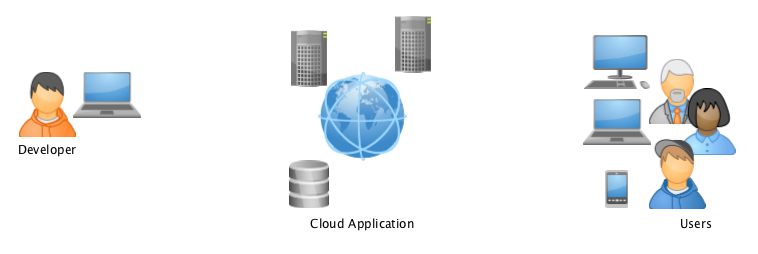
\includegraphics[width=12cm]{FOverview.png}

\only<2->{
Development options:
\begin{itemize}
\item<3-> \only<3>{Develop on Production Servers}\only<4->{\sout{Develop on Production Servers}} \only<4->{{\color{red} NO}}
\item<5-> Clone Cloud Environment \only<6->{{\color{orange} Expensive}}
\item<7-> Local copy of the environment \only<8->{{\color{orange} Expensive}}
\item<9-> Local virtualised environment \only<10->{{\color{green} Cheap}} \only<11->{{\color{orange} Testable?}}
\end{itemize}
}
\end{frame}

\begin{frame}[t]
\frametitle{Overview}

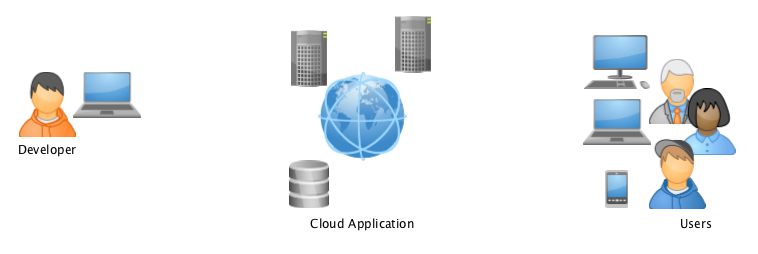
\includegraphics[width=12cm]{FOverview.png}

Challenges:
\begin{itemize}[<+->]
\item Keep Local Development environment and Cloud deployment environments similar
\item Test environment $\neq$ Development environment
\item A single way to configure all environments (and to store different configurations)
\end{itemize}
\end{frame}

\begin{frame}[t]
\frametitle{In this lab\ldots}

\only<1>{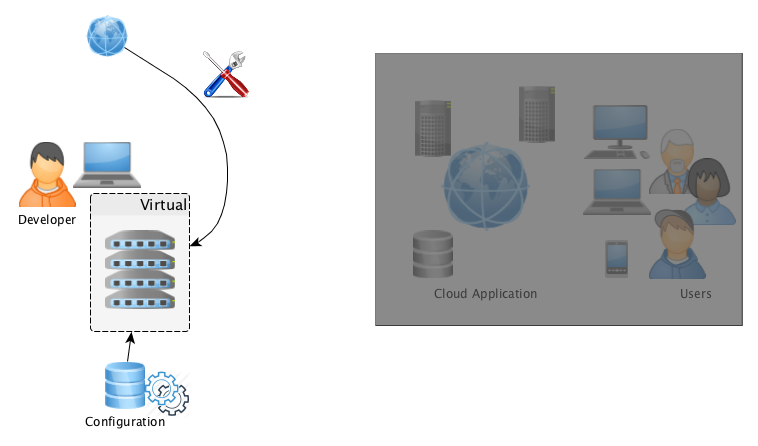
\includegraphics[width=12cm]{FLocal.png}}
\only<2>{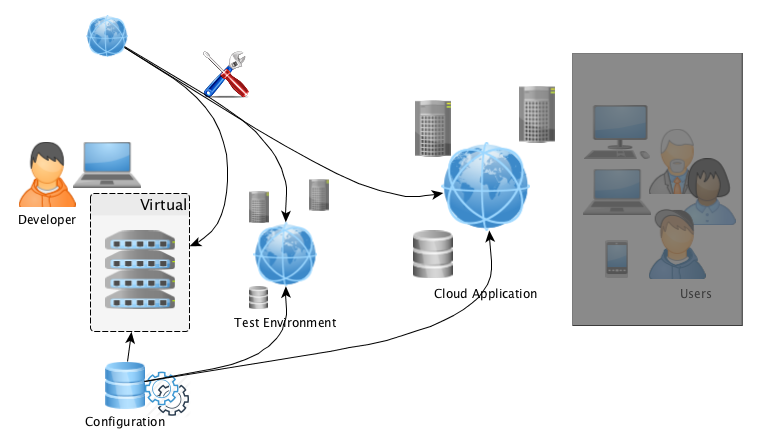
\includegraphics[width=12cm]{FTestDeploy.png}}
\only<3->{
\includegraphics[width=12cm]{FLabOverview.png}}

\begin{tabular}{*{4}{p{2.85cm}}}
\only<3->{Virtualisation} &
\only<4->{Provisioning} &
\only<5->{Multi-Machine} &
\only<6->{Deployment}\\
\end{tabular}
\end{frame}



% -----------------------------


%% All of the following is optional and typically not needed. 
%\appendix
%\begin{frame}[allowframebreaks]
%  \frametitle{For Further Reading}
%    
%  \begin{thebibliography}{10}
%    
%  \beamertemplatebookbibitems
%  % Start with overview books.

%  \bibitem{Author1990}
%    A.~Author.
%    \newblock {\em Handbook of Everything}.
%    \newblock Some Press, 1990.
%     
%  \beamertemplatearticlebibitems
%  % Followed by interesting articles. Keep the list short. 

%  \bibitem{Someone2000}
%    S.~Someone.
%    \newblock On this and that.
%    \newblock {\em Journal of This and That}, 2(1):50--100,
%    2000.
%  \end{thebibliography}
%\end{frame}

\end{document}


